\documentclass[twocolumn]{aastex62}
%\documentclass{aastex62}
%\documentclass{emulateapj}

%\usepackage{apjfonts}
\usepackage[T1]{fontenc}
\usepackage{color}
\usepackage{amsmath,amstext}
\usepackage{hyperref}
\usepackage{natbib}
\usepackage{subcaption}
% Our definitions

\newcommand{\code}[1]{\texttt{#1}}
\newcommand{\mesa}{\code{MESA}}
\newcommand{\MESA}{\mesa}
\newcommand{\FLASH}{\code{FLASH}}

% Our definitions
\newcommand\beq{\begin{equation}}
\newcommand\eeq{\end{equation}}
\newcommand{\mini}{M_{\rm ini}}
%\newcommand{\Msun}{\ensuremath{\unitstyle{M}_\odot}}


\newcommand{\Msun}{\ensuremath{{\rm M}_\odot}}
\newcommand{\Mj}{\ensuremath{{\rm M}_{\rm J}}}
\newcommand{\mso}{\ensuremath{{\rm M}_\odot}}
\newcommand{\rso}{\ensuremath{{\rm R}_\odot}}
\newcommand{\kms}{\ensuremath{{km}\,\second^{-1}}}
\newcommand{\Rsun}{\ensuremath{{\rm R}_{\odot}}}
\newcommand{\second}{{s}}


%\received{January 8th 2019}
%\submitjournal{ApJ}

 
\shorttitle{Planetary Engulfments}
\shortauthors{Cantiello et al.}
  
\begin{document}
\title{Simulations of Planetary Engulfment in MESA: Hot Jupiters}


\author[0000-0002-8171-8596]{Matteo Cantiello et al.}
\affiliation{Center for Computational Astrophysics, Flatiron Institute, 162 5th Avenue, New York, NY 10010, USA}
\affiliation{Department of Astrophysical Sciences, Princeton University, Princeton, NJ 08544, USA}

\author{Mike Y. M. Lau}
\affiliation{Center for Computational Astrophysics, Flatiron Institute, 162 5th Avenue, New York, NY 10010, USA}
\affiliation{School of Physics and Astronomy, Monash University, Clayton, Victoria 3800, Australia}
\affiliation{OzGrav: The ARC Centre of Excellence for Gravitational Wave Discovery, Australia}

\author[0000-0001-5048-9973]{Adam S. Jermyn}
\affiliation{Center for Computational Astrophysics, Flatiron Institute, 162 5th Avenue, New York, NY 10010, USA}

\author{Orsola de Marco}
\affiliation{Department of Physics & Astronomy, Macquarie University, Sydney, NSW 2109, Australia}

%\author{Melinda Soares-Furtado}
%\affiliation{Department of Astrophysical Sciences, Princeton University, Princeton, NJ 08544, USA}



%\author{Morgan MacLeod}
%\affiliation{Harvard-Smithsonian Center for Astrophysics, 60 Garden Street, Cambridge, MA 02138, USA}
%\altaffiliation{NASA Einstein Fellow}





\correspondingauthor{Matteo Cantiello}
\email{mcantiello@flatironinstitute.org}


\begin{abstract}
Many sun-like stars have planets orbiting in close enough orbits to be engulfed when their host stars ascend the giant branch.  We present one dimensional calculations of planetary engulfments using the Modules for Experiments in Stellar Astrophysics (\MESA) software instrument. 
When a planet enters the stellar envelope, orbital energy is dissipated via hydrodynamic or gravitational drag. We self-consistently track the orbital evolution of the engulfed planet, and the corresponding energy injection. We determine the maximum depth of planetary engulfment assuming disruption occurs when the ram pressure integrated over the cross section of the planet approaches its binding energy. The dissipation of orbital energy in the stellar envelope can change the entropy profile of the star and temporarily shut-off convection. This can have important consequence for the stellar ability to transport the injected energy outwards. 
Our calculations allow to follow the evolution of stellar structure and luminosity of the primary star, and while providing only a rough approximations of the complex engulfment process, unlike multi-dimensional calculations they can be used to rapidly span the vast parameter space of star-planet systems. The results we present outline the parameter space on the giant branch where interaction with planetary companions leads to significant energetic perturbations of host stars. Stellar transients with duration of xx months and brightness changes of up to yy magnitudes  are expected in the subgiant and lower  giant branch. On the other hand rocky planets or planets on distant orbits, lead to minor perturbations of their host stars. 
We tentatively discuss rates and detectability of such events by transient surveys like ZTF and the Vera Rubin Observatory / LSST. 
\end{abstract}  

\keywords{}

\section{Introduction}\label{sec:introduction}

Planetary Engulfments Plan:

\begin{itemize}
    \item Determine role of density choice (average etc)
    \item Add Tangential and Vertical Velocity Tracking
    \item Add gaussian energy distribution
    \item Add orbital energy left at planetary destruction
    \item Check convection treatment during rapid phases (PISN treatment from Pablo)
    \item Use gold tolerances and dedt form of energy conservation [done]
    \item Rerun models
    \item Check dependency on energy deposition Type 
    \item Do a convergence study
\end{itemize}


- Plots (for 3 cases): 


\begin{itemize}
    \item Rp vs Rb given a typical structure and for different planets
(10Mj, Mj, Uranus, Earth) 
    \item Lightcurve
    \item Kippenhahn Diagram
    \item Kipp diagram with en injected (as f of radius)
    \item Stellar Radius and Planet location vs time
    \item L deposited vs L star as function of time
    \item Trajectory Plots
    \item $(vtan^2+vrad^2)^{0.5}$ / cs as function of time
    \item Comparison to V1309 Sco (?)
    \item Comparison of a couple of cases to HRD plot of MacLeod etc.
    \item Comparison to Orsolas results
\end{itemize}


Villaver  Livio (2009) calculated how tidal interactions in the subgiant and giant stages can lead to the final engulfment of the close-in planets. Likewise, Villaver et al. (2014) have analyzed the effects of the evolution of the planet’s orbital eccentricity, mass-loss rate, and planetary mass on the survivability of planets orbiting stars with masses above 1.5. They
conclude that the planet mass is a key parameter for the engulfment during the subgiant phase, with the more massive planets more likely falling into the stellar envelope during this phase (for
the same initial orbital parameters). Also, planets located at 2-3
R, when the star begins to leave the main sequence, may suffer orbital decay from the influence of stellar tides. Any planet closer than this orbital distance may be engulfed by the star in the subgiant phase. \citet{Lillo-Box:2016} showed observationally that this is indeed the case, and that  the closest-in planets are 
engulfed by their host as it evolves to the red giant branch.  

\section{Model}
We performed 1D calculations of evolved low-mass stars undergoing planetary engulfments. Our models are calculated
using revision 15140 of \MESA\ (Modules for Experiments in Stellar
Astrophysics) \citep{Paxton:2011,Paxton:2013,Paxton:2015,Paxton:2018,Paxton:2019}. Below we describe the assumptions and features of our models, including the extensions to the code required to follow the engulfment process. 


A planet can be engulfed by its star for a number of reasons, including dynamical interactions, tides, Roche-Lobe Overflow (RLOF), and magnetic torques \citep[e.g.][]{Metzger_2012,Strugarek:2017,Stephan:2018,Benbakoura:2019}. Some of these processes become more significant when the stellar companion evolves past its main sequence. Ultimately, engulfments are inevitable for planets with orbital separations smaller than the maximum radial extension obtained by the star during its red giant evolution \citep[e.g.][]{MacLeod2018}.


\begin{figure} \centering
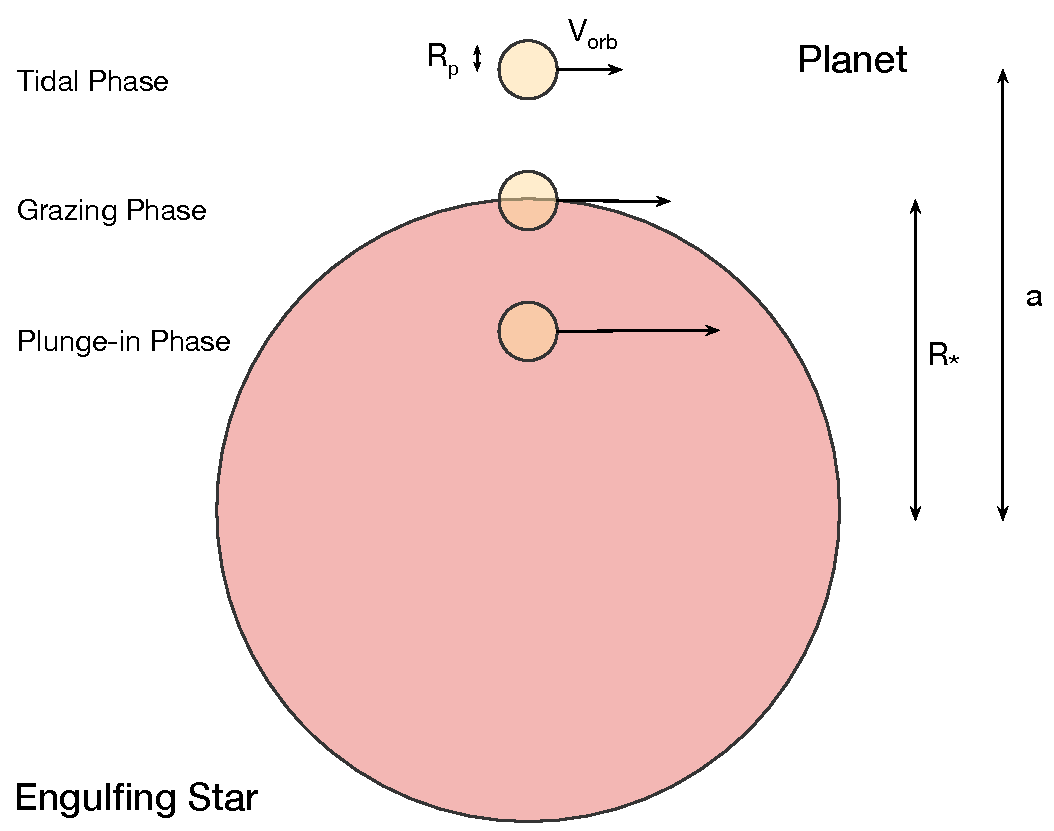
\includegraphics[width=\linewidth]{figures/sketch.pdf}
\caption{Outline of our model.}
\label{fig:sketch}
\end{figure}


Irrespective of the  process that led to such configuration, in our models we just start with a planet grazing its stellar companion on a circular orbit.
Specifically, we consider a system composed of a star of mass $M_*$, radius $R_*$, and luminosity $L_*$,  and a lower-mass companion of mass $M_{\rm p} \ll M_*$ and radius $R_{\rm p}$ on a circular orbit with separation $a$. 
%=R_*+R_{\rm p}$. 
The orbital velocity of the planet is 
\beq\label{eq:vorb}
v_{\rm orb} =  \left[\frac{G (M_*(a) +M_{\rm p})}{a} \right]^{1/2} \simeq \left[\frac{GM_*(a)}{a} \right]^{1/2},
\eeq
where $M_*(a)$ is the stellar mass enclosed at a distance $a$ from the stellar center, with $M_*(a) = M_*$ if $a \geq R_*+R_{\rm p}$.  The orbital energy of the system is  
\beq\label{eorb}
E_{\rm orb}(a) = \frac{G M_*(a) M_{\rm p}}{2 a},
\eeq
and as the companion orbits inside the envelope of the primary, there are a number of processes that can extract and dissipate part of this energy. These include tides, Roche-Lobe Overflow (RLOF), hydrodynamic and gravitational drag, accretion and magnetic fields. In our models we will focus on the effects of drag and tides, which are the most important processes for studying the engulfment of Hot Jupiters around post main sequence stars (see Sec.~\ref{sec:disruption}).  

%with associated orbital period
%\beq\label{porb}
%P_{\rm orb} = 2 \pi \left[\frac{R_*^3}{G (M_*+ M_{\rm p})}\right]^{1/2}. 
%\eeq
%\subsection{Energy Dissipation and Orbital Decay}
%As the companion moves into the envelope of the primary, there are a number of processes that can dissipate part of its orbital energy. These include tides, Roche-Lobe Overflow (RLOF), aerodynamic and gravitational drag, accretion and magnetic fields. For the rest of the paper we will focus on the role of drag and tides, as these process contribute the most in the case of a planetary engulfment [JUSTIFY]. 

\subsection{Hydrodynamic and Gravitational Drag}
A planet moving inside a star experiences both a
gravitational and hydrodynamic drag. The hydrodynamic drag force is produced by the gradient of the surrounding gas ram pressure:
\begin{equation}
F_{\rm hd}= C_d\, \rho\, v_{\rm p}^2\,\pi R_{\rm p}^2,
\label{eqQ:hydrodrag}
\end{equation}
where $v_{\rm p}$ is the planet's relative velocity with respect to the gas flow, $R_{\rm p}$ is the radius of the  planet, $\rho$ is the local density of the stellar gas at the location of the planet, and $C_d$ is a dimensionless drag coefficient. 

On the other hand, the gravitational drag is caused by gravitational forces between the planet and its wake in the ambient medium. A good approximation for this force is \citep[e.g.][]{Iben:1993}:
\begin{equation}
F_{\rm gd}= \zeta\, \rho\, v_{\rm p}^2\,\pi R_{\rm A}^2,
\label{eq:gravdrag}
\end{equation}
where $\zeta$ is a drag coefficient of order unity that depends on the Mach number \citep{Shima:1985,Ostriker:1999}, 
and $R_{\rm A}$ is  the impact parameter below which matter is accreted \citep{Bondi:1952,Iben:1993}:
\begin{equation}
R_{\rm A}=\frac{2GM_{\rm p}}{v_{\rm p}^2+c_s^2},
\label{eq:rabondi}
\end{equation}
where $c_s$ is the 
sound speed. The work of \citet{MacLeod:2015,MacLeod:2017} shows that the drag coefficient rises in flows with steeper density gradients, and also tend to be larger in more compressible flows. 

For simplicity in our models we calculate the resulting drag force acting on a planet as
\begin{equation}
F_{\rm d}= \rho v_{\rm orb}^2 \,A 
% A = \pi~{\rm max}(R_{\rm p}, R_{\rm A})^2,
\label{eq:rabondi}
\end{equation}
where $A = \pi\,{\rm max}\,(R_{\rm p}, R_{\rm A})^2$, we assumed a maximal value of the relative velocity equal to the Keplerian orbital velocity of the planet (Eq.~\ref{eq:vorb}), and a constant value for both the hydro and gravitational drag coefficients ($C_d = \zeta = 1$). We neglect both possible changes in the size of the planetary radius during the inspiral, as well as changes in the values of the drag coefficients as function of Mach number \citep{Ostriker:1999} and Reynolds number\footnote{At very high Reynolds numbers the drag is often essentially independent of the Reynolds number \citep[see e.g.][]{Munson:2005}.}. For the value of the density $\rho$, we take the average of the stellar density in the region of size $2A$ at the location of the planet $a$. Note that in the case of planetary companions interacting with stars, the geometric cross section $\pi R_{\rm p}^2$ is almost always larger than the gravitational cross section $\pi R_{\rm A}^2$ (Lau et al. In prep.). 

The rate of energy dissipation due to drag forces is 
\begin{equation}\label{eq:de}
\frac{dE}{dt} = - A\, \rho \,v_{\rm orb}^3 .
\end{equation}
  %\citep[e.g.][]{MacLeod2018}. 
  %We also assume that  $v_{\rm rel}=v_{\rm orb}$ during most of the engulfment process, which is a good assumption even in the last phases of an engulfments, since the keplerian and free-fall velocity are approximately the same. 
which together with Eq.~\ref{eq:vorb} allows to calculate the spiral-in evolution, e.g. \citet{Tylenda:2006}. 
\begin{equation}\label{eq:dr}
\frac{da}{dt} \simeq -\frac{2A}{M_{\rm p}} \rho \sqrt{G M_*(a)\, a},
\end{equation}
%where we also adopted $M_* \gg M_2$. 

We keep track of equations \ref{eq:de} and \ref{eq:dr} in a 1D MESA calculation to determine the energy injection rate inside the stellar envelope, as well as the orbital evolution of the location of the engulfed companion, relative to the primary center.  
We are able to follow the evolution of the primary star as function of the different parameters of the engulfment event ($M_*, R_*, M_{\rm p}, R_{\rm p}$). While this is a very simplified model, it allows a relatively quick estimate of the expected luminosity and duration of transient events associated with the engulfment of planetary companions, at least in the case where the emission is dominated by the heating of outer layers of the star (See sec.~\ref{sec:emission}).
%%%%%% MC:
% the location $r$ inside the primary as function of time. This is function of the local density $\rho$ at location $r$, the radius of the companion $R_2$ and the orbital velocity $v_{\rm orb}$ (we assume here $v_{\rm orb} = v_{\rm orb,2} \approx v_{\rm orb,2} - v_{\rm orb,1}$).

\subsection{Tides}
We calculate the effect of tides using the equilibrium tide model of \citet{Hut:1981} in the formulation of \citet{Eggleton:1998}. 
The evolution of the orbit under the influence of tidal dissipation is given by 
\begin{equation}\label{eq:dr_tides}
\frac{da}{dt} = -\frac{a}{T_*},
\end{equation}
with the tidal timescale calculated as 

\begin{equation}\label{eq:t_tides}
T_* = \frac{1}{9}\,\frac{M_*}{(M_*+M_{\rm p})M_{\rm p}} \frac{a^8}{R_*^{10}} \frac{1}{\sigma_*}.
\end{equation}
Here $\sigma_*$ is the stellar tidal dissipation factor, with $\sigma_* = \overline{{\sigma}}_* \, \sigma_0$ where the dimensional scaling factor $\sigma_0$ is given by $(G\mso/\rso^7)^{1/2} = 6.4\times10^{-59}\, {\rm g}^{-1} \, {\rm cm}^{-2}\, {\rm s}^{-1}$ \citep{Hansen:2010}. In our models  we adopted an observationally--derived calibration of the tidal dissipation factor from \citet{Hansen:2012}, $\overline{{\sigma}}_* = 10^{-9}$, which is appropriate for planets orbiting giant stars.   


Note that in principle this formalism breaks down for $a<R_*$. However, since in evolved stars the mass is strongly concentrated towards the center, to first approximation we can ignore the effects of material outside the planet's orbit. Therefore, we use eq.~\ref{eq:t_tides} with $M_*$ equal the enclosed stellar mass $M_*(a)$, and with the stellar radius $R_* = a$.

As we will see, the effect of tides when $a<R_*$ is usually negligible compared to drag forces.



\subsection{Energy Deposition}
As the planet spirals in, we inject in the stellar structure the energy dissipated by drag forces as internal energy \citep[e.g.][]{Taam:1978,Clayton:2017,Fragos:2019}. In \MESA\ this can be easily done using the \code{other\_energy} hook. We spread the energy uniformly  in the gas contained in a region of size $2A$ centered around the location of the planet $a$. This way we can follow the back-reaction of the stellar structure to the planetary engulfment, with the orbital evolution affected by the energy deposition mostly via changes in the local gas density (Eq.~\ref{eq:dr}). We do not include the heating effect of tidal dissipation, as this is usually negligible compared to drag heating. 
We follow the evolution of the system until the engulfed planet is destroyed. At that point we stop injecting energy and let the star relax for a time equal to its thermal timescale. 



\subsection{Planet Destruction}\label{sec:disruption}
Planets orbiting close to their stars can be destroyed by tidal forces or RLOF even before getting engulfed \citep[e.g.][]{Metzger_2012}. In particular, \citet{Metzger_2012} found that the fate of a planet is set by the ratio of its mean density $\overline{\rho}_{\rm p}$ to the stellar mean density $\overline{\rho}_{\rm *}$. If $\overline{\rho}_{\rm p}/\overline{\rho}_{\rm *} \gtrsim 5$, then the planet plunges below the stellar atmosphere before it is destroyed by tides or accreted.  
Here we only consider this case (direct impact), which is mostly relevant for merger events between planets and  post main sequence stars. For a Hot Jupiter around a $1\mso$ star, $\overline{\rho}_{\rm p}/\overline{\rho}_{\rm *} \gtrsim 5$ is satisfied as long as $a = R_* + R_{\rm p} \gtrsim 1.71\, \rso$. Therefore planetary destruction occurs inside the star for  post main sequence engulfments  of Hot Jupiters (see Fig.~\ref{fig:hrd}). 

%Here we consider the case in which a planet survived tidal interaction with its host star companion and is undergoing an engulfment event. There are two main processes that can lead to the disruption of the planet inside the star: ablation and stripping.

One potential candidate for planetary disruption during an engulfment event is ablation, basically a slow peeling of the planetary surface. However, \citet{Jia_2018} found this process to be ineffective due to the large density ratio between the planet's surface and the stellar envelope. Even in the case of a low density gas planet, this process is not efficient because the low entropy atmosphere gets compressed by the ram pressure, creating a sort of protective layer that halts the ablation process. 

According to \citet{Jia_2018} the most important process is instead a global deformation that occurs when the ram pressure integrated over the cross section of the planet approaches its binding energy. This process leads to splitting, fragmentation and eventually total destruction of the planet when 

\beq  \mathcal{F} \equiv \frac{\rho_{\rm ext} \, v^2}{\bar{\rho}_{\rm p} \, v^2_{\rm esc}} \approx 1, \label{eq:jia}\eeq

where $\rho_{\rm ext}$ is the density of the flow around the planet, $v$ its relative velocity, $\bar{\rho}_{\rm p}$ is the average density of the planet and $v_{\rm esc}$ the escape velocity from its surface. 
This criterion is simple to evaluate, as $\mathcal{F}$ increases monotonically while a planet plunges into its host star, and we adopted it in our models to establish the location of planetary disruption. 
%After the planet is destroyed, we stop injecting energy and allow the star to relax for a thermal timescale.

\subsection{Time Step Limits}\label{sec:time_steps}
To ensure that \MESA\ is properly resolving the rapid phases of evolution associate with the engulfment process, we enforce tighter time-stepping conditions compared to the ones already present \citep{Paxton:2011}. In particular, we use a criterion that reduces the time step until the relative change in the orbital separation is smaller than a user-defined tolerance value. Typical values are $da/a = 10^{-4}$ during  tidal evolution, 
and $da/R_{\rm p} = 10^{-3}$ and $10^{-2}$ during the grazing and the plunge-in phase, respectively (see Sec.~\ref{sec:phases} for a more detailed discussion of these phases). 



\begin{figure}
\centering
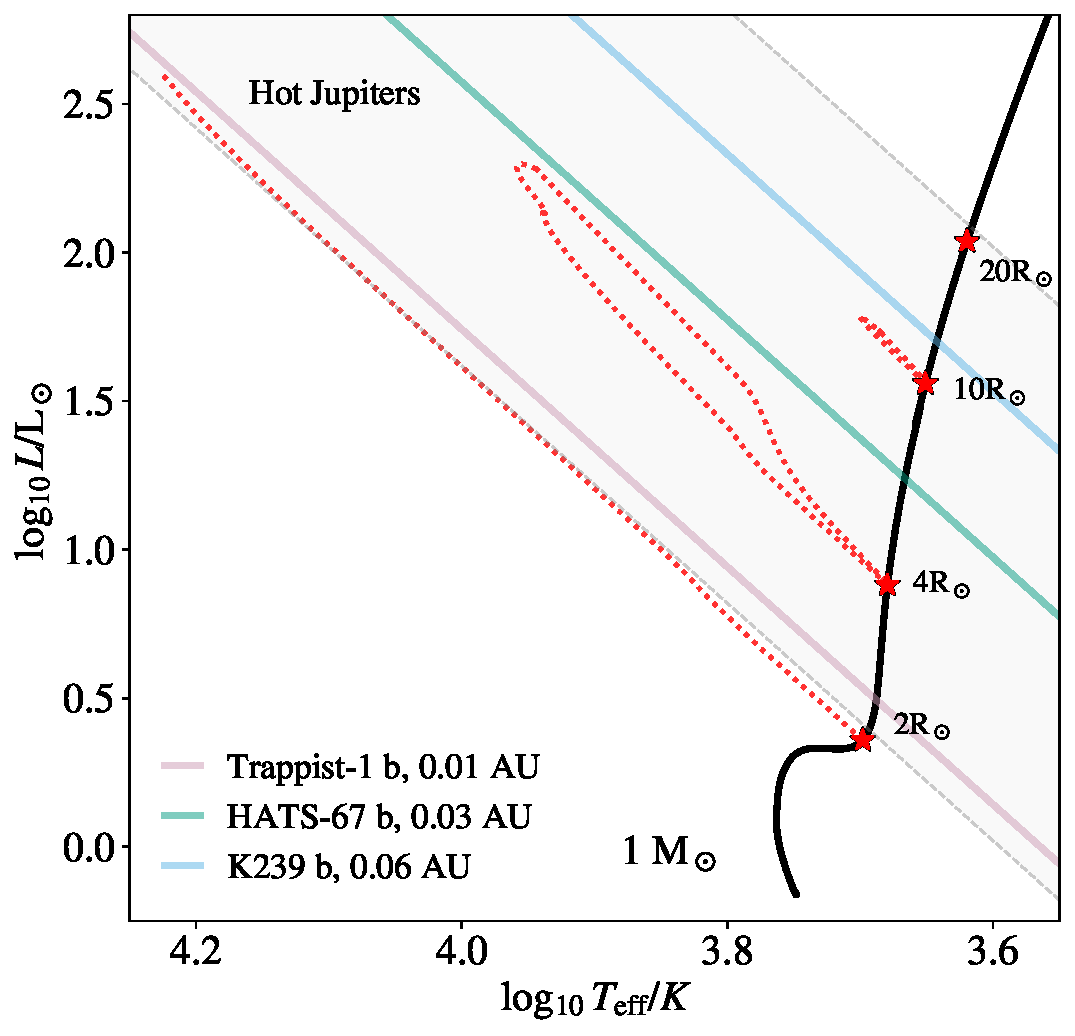
\includegraphics[width=.992\columnwidth]{figures/hrd.pdf}
\caption{Evolution of our 1$\Msun$ model on the Hertzsprung-Russel diagram. The gray area shows the typical orbital separation of Hot Jupiters, with a few specific objects shown (solid lines). The initial orbital separation of our planetary engulfment runs are shown by the star symbols. The evolution of the models during the engulfment phase is shown by the red, dotted lines.}
\label{fig:hrd}
\end{figure}



\begin{figure*}
\centering
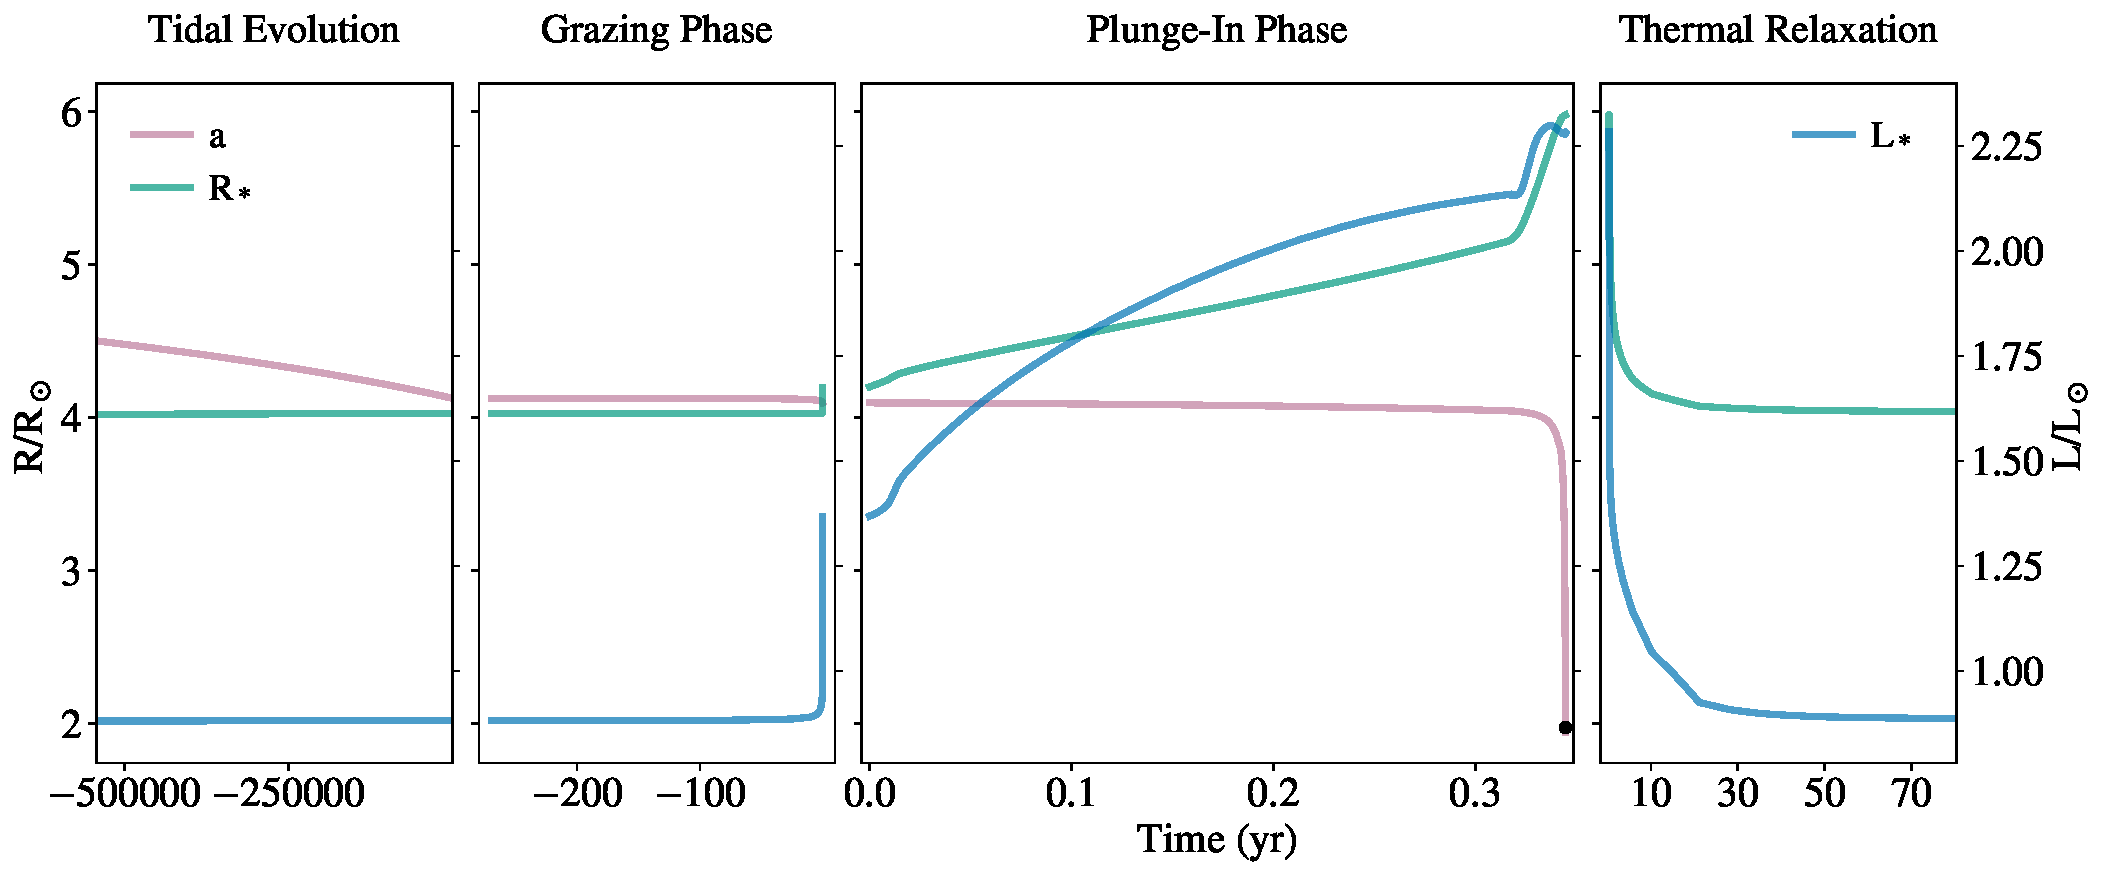
\includegraphics[width=\textwidth]{figures/evolution3.pdf}
\caption{Different phases of evolution during the engulfment of a planet with Jupiter mass (0.001$\Msun$) and Jupiter radius (0.1$\Rsun$) around a red giant star with mass 1$\Msun$ and radius 4$\Rsun$.}
\label{fig:evolution}
\end{figure*}
 
 
\section{Results}
In our models, planetary engulfments proceed through four different phases characterized by different timescales. To resolve these phases we need to enforce tighter time-step conditions than usually implemented in \MESA, as discussed in sec.~\ref{sec:time_steps}.
  
\subsection{Engulfment Phases}\label{sec:phases}
We initialize our calculations starting from a 1$\Msun$ model with solar metallicity (Z=0.02). This model was evolved past the end of core hydrogen burning and onto the giant branch, and we selected different post main sequence starting points corresponding to radial extensions of $R_* = 2, 4, 10,$ and $ 20~\Rsun$ (see Fig.~\ref{fig:hrd}). A planetary companion with $M_p = 0.001\Msun$ and $R_p = 0.1\Rsun$, roughly corresponding to Jupiter's values,  is initialized with $a = R_* + da$, so that tides can rapidly shrink the orbit (see Eq.~\ref{eq:t_tides}). Since here we neglect the effects of RLOF (see Sec.~\ref{sec:disruption}), this tidal phase lasts until the planet, or the planet's Bondi sphere, reaches the outer layers of the star. 
%The timescale of this phase is long, and dictated by Eq.~\ref{eq:t_tides}. 


At this point we start injecting orbital energy into the stellar region occupied by the planet (or the planet's Bondi sphere, whichever is larger). Since the density is very low in the outer layers of the star, initially the amount of orbital energy dissipated via hydrodynamic or gravitational drag is not very large. Moreover, the energy deposition inflates the outer layers, decreasing their average density. The result in a fairly long evolution in this grazing phase, of order $10^2-10^3$ yr (see Fig.~\ref{fig:evolution} and \ref{fig:spiral20}). During the grazing phase we track the geometric cross section of the planet or the planet's Bondi sphere with the star (Fig.~\ref{fig:sketch}). We assume a plane parallel approximation, which is good as long as $R_{\rm p} \ll R_{\star}$. Eventually the planet gets engulfed because its orbit decays and because of the host star's inflation, which results in heating and associated brightening of low-optical depth, outer stellar layers. We track the engulfment fraction and calculate the area entering Eq.~\ref{eq:de} accordingly. We define the end of the grazing phase when the engulfment fraction reaches the value of one. At this point the plunge-in phase begins. 

During the plunge-in phase the orbital velocity and local density grow, leading to a substantial increase in the luminosity deposited in the outer stellar layers. The radial migration of the in-falling planet now occurs on the much shorter, dynamical timescale. 
While the injected energy is initially radiated away efficiently, as the planet plunges into deeper, higher optical depth layers, the heating energy gets progressively trapped. This occurs as the thermal timescale of the overlying material becomes longer than the plunge-in timescale.
While in the grazing phase all the injected energy during a time-step emerges immediately as stellar luminosity, as the planet drifts inward the amount of injected luminosity becomes larger than the total stellar luminosity (Fig.~\ref{fig:luminosities}). The extra energy is thermalized and trapped in deeper layers, emerging only on longer timescales. This process determines the bolometric brightness increase in our models, with a peak in stellar luminosity occurring toward the end of the plunge-in phase (see Fig.~\ref{fig:evolution}). This peak usually occurs right before the planet is destroyed: As the relative velocity and average density of the flow increase, the ram pressure integrated over the cross section of the planet approaches its binding energy. The condition for planetary destruction is met ($\mathcal{F} = 1$, see Eq.~\ref{eq:jia}). At this point we stop tracking the planet orbit and injecting energy into the stellar structure (black dot in Fig.~\ref{fig:evolution}). This determines the end of the plunge-in phase. The maximum penetration point of the planet depends mostly on the radius of the star, with planets engulfed in more compact stars being destroyed 
in shallower layers than more evolved, larger stars. This is due to the planet's larger orbital velocity coupled with a lower average density of the stellar envelope. In the case of an Hot Jupiter engulfed by a $4\Rsun$ red giant, we determine a destruction radius of about 1.95$\Rsun$. For the same planet plunging into a $20\Rsun$ red giant, the destruction radius is 0.45$\Rsun$ (see Fig.~\ref{fig:spiral4} and \ref{fig:spiral20}). These radii usually correspond to the lower bottom of the convective envelope. 

After the planet's destruction, we lift the time-step restrictions and allow the star to thermally relax. During this thermal relaxation phase,  all the deposited energy that was trapped within the stellar envelope is released as stellar luminosity. This phase lasts on the order of the thermal timescale of the affected envelope (see e.g. right-most panel in Fig.~\ref{fig:evolution}, where we only show the first ~80 years of such evolution). At the end of this phase the stellar radius and luminosity return to pre-engulfment values. 


\begin{figure}
\centering
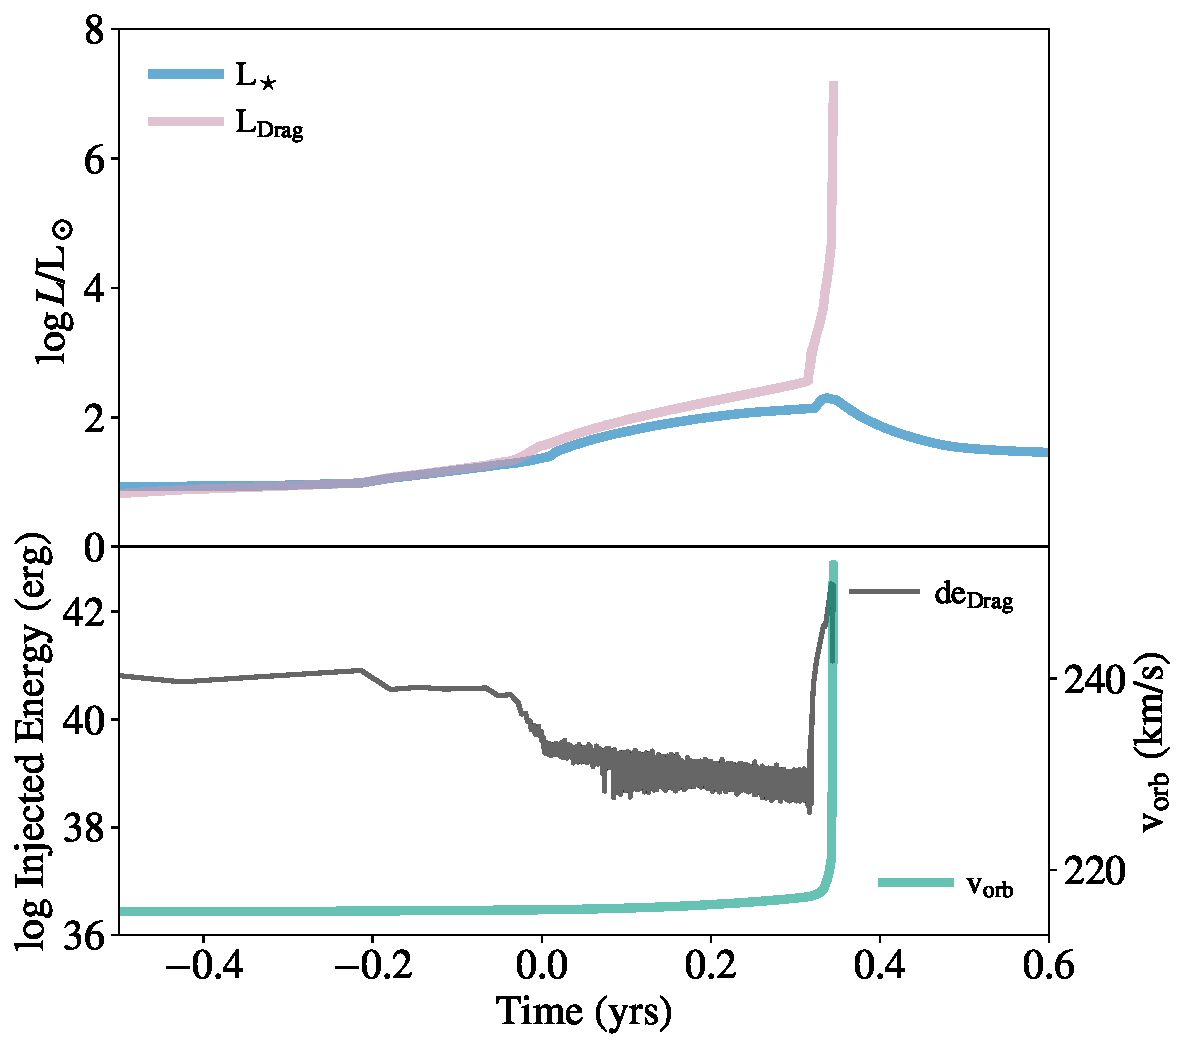
\includegraphics[width=.992\columnwidth]{figures/luminosities.pdf}
\caption{Stellar bolometric luminosity and drag luminosity as function of time, from the late phases of grazing evolution, through the plunge-in phase, and the beginning of thermal relaxation. The lower panel shows the amount of drag energy injected per time-step, as well as the evolution of the orbital velocity of the planet.}
\label{fig:luminosities}
\end{figure}

\begin{figure}
\centering
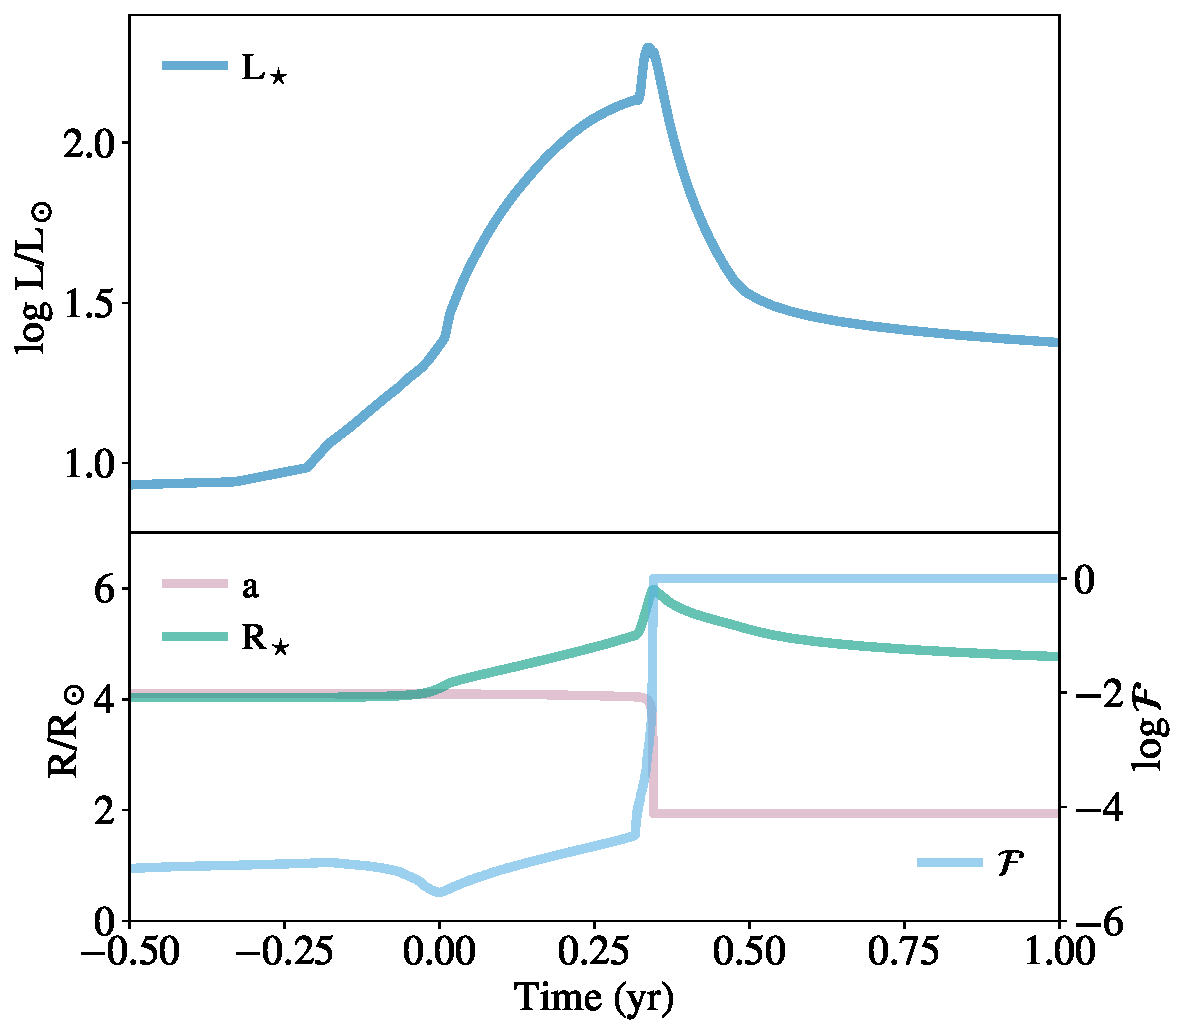
\includegraphics[width=.992\columnwidth]{figures/lightcurve.pdf}
\caption{Evolution of bolometric luminosity of the star from the late phases of grazing evolution, through the plunge-in phase, and the beginning of thermal relaxation.}
\label{fig:lightcurve}
\end{figure}


%\subsubsection{Tidal Phase}
%\subsubsection{Grazing Phase}
%\subsubsection{Plunge-in Phase}
\subsection{Evolution of the Host Star}
The host star reacts to the energy injection by heating up and evolving on the Hertzsprung-Russel (H-R) Diagram following lines of approximately constant radius (see Fig.~\ref{fig:hrd}). A modest radial expansion still occurs, especially in models on the lowest part of the red giant branch. These models are affected the most by the engulfment process, while models that engulfed a planetary companion beyond the luminosity bump (R$_\star\gtrsim$ 10\Rsun\ in our 1\Msun\ model) endure very small variations of their H-R Diagram position. This is in agreement with the predictions of \citet{MacLeod2018}, who used scaling relations to map out the parameter space along the giant branch where interaction with planetary companions could lead to significant energetic disturbance of host stars.

As previously discussed, the relaxation of stars that have engulfed a planet occurs on the thermal timescale of the affected envelope. So even if the brightest part of the transient lasts only for a few months, it might still be possible to observe the slow dimming that occurs during the thermal relaxation phase \citep{Metzger_2012}. 

Besides changing the stellar luminosity, the engulfment might also affect the mass loss and rotational evolution of the star \citep{Privitera:2016a,Privitera:2016b}, as well as its surface composition \citep{Soares:2021} and magnetism \citep{Privitera:2016bf}. While we neglected these effects in our simplified models, we discuss the possible impact of these effects in Sec.~\ref{sec:discussion}.

%fairly mild (e.g. 50\% for the 4\Rsun\ model, and 10\% for the 10\Rsun\ model) 

\begin{figure*}
\centering
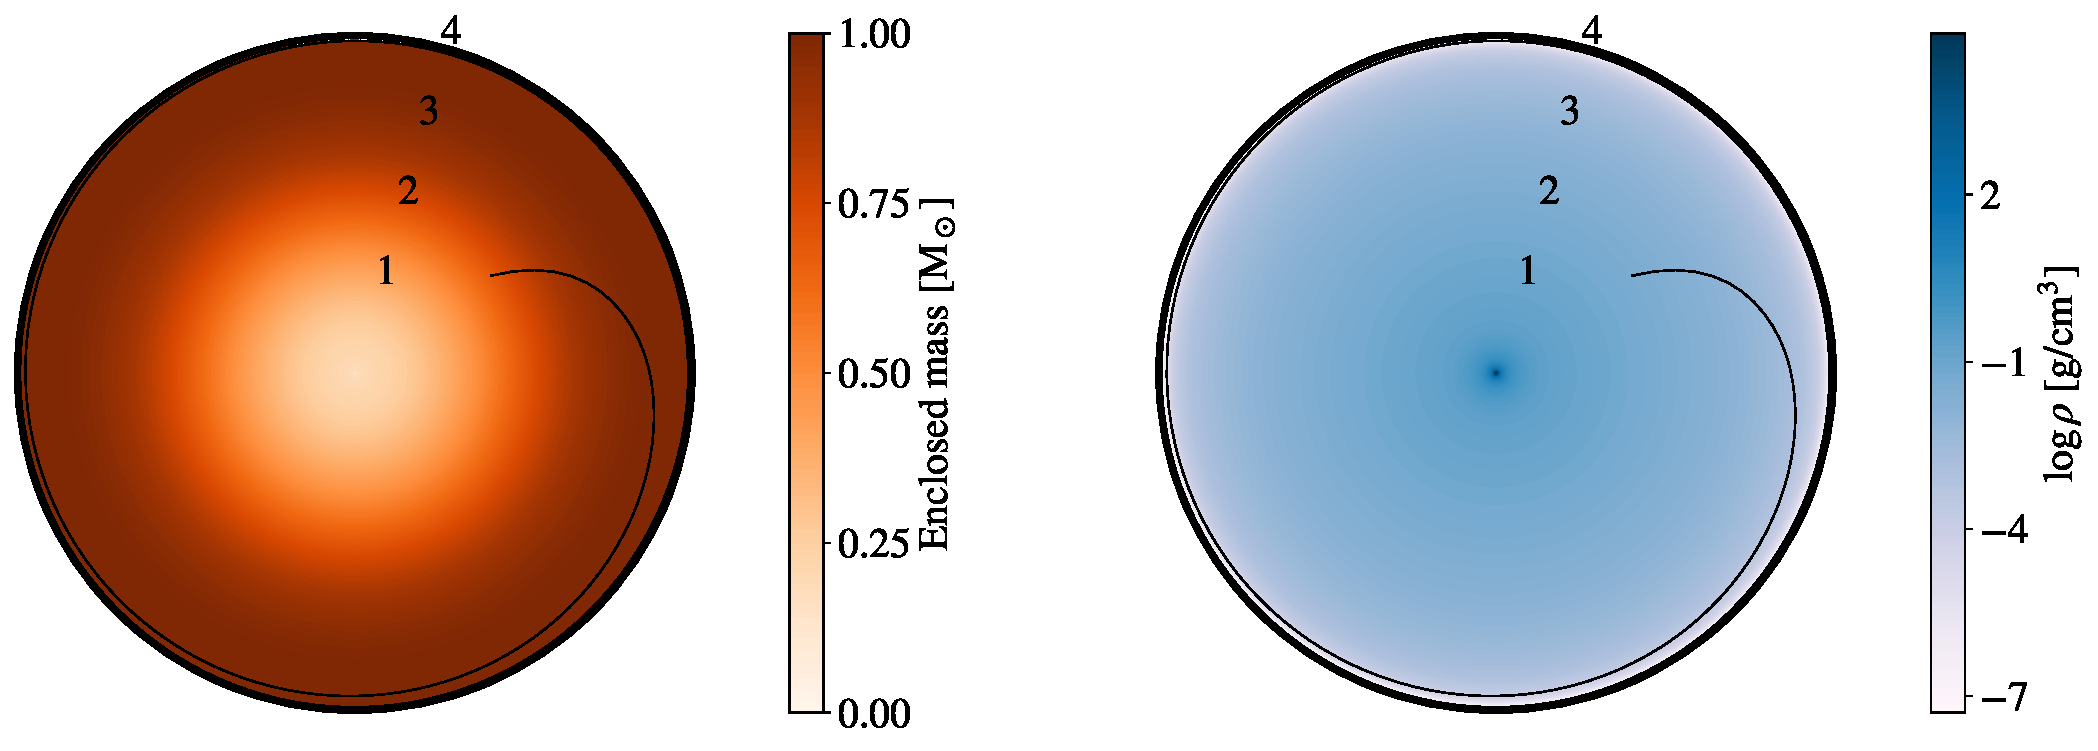
\includegraphics[width=\textwidth]{figures/polar_mj_r4.pdf}
\caption{Engulfment of a planet with Jupiter mass and radius around a red giant star with mass 1$\Msun$ and radius 4$\Rsun$.}
\label{fig:spiral4}
\end{figure*}


\begin{figure*}
\centering
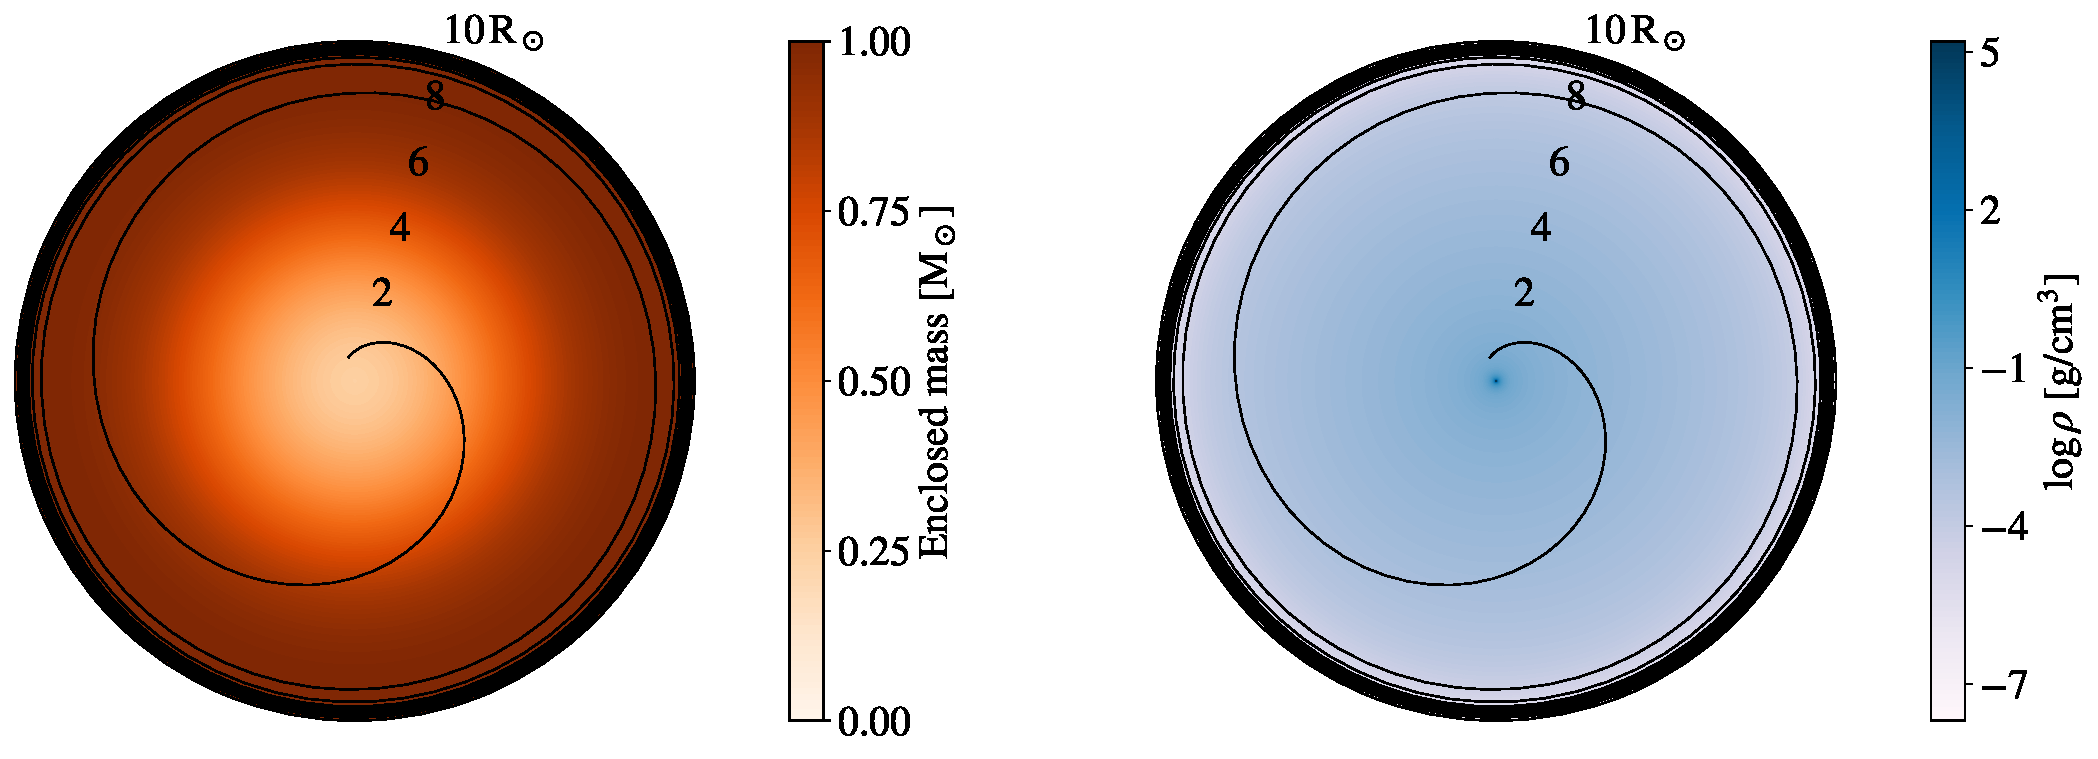
\includegraphics[width=\textwidth]{figures/polar_mj_r10.pdf}
\caption{Engulfment of a planet with Jupiter mass and radius around a red giant star with mass 1$\Msun$ and radius 10$\Rsun$.}
\label{fig:spiral10}
\end{figure*}


\begin{figure*}
\centering
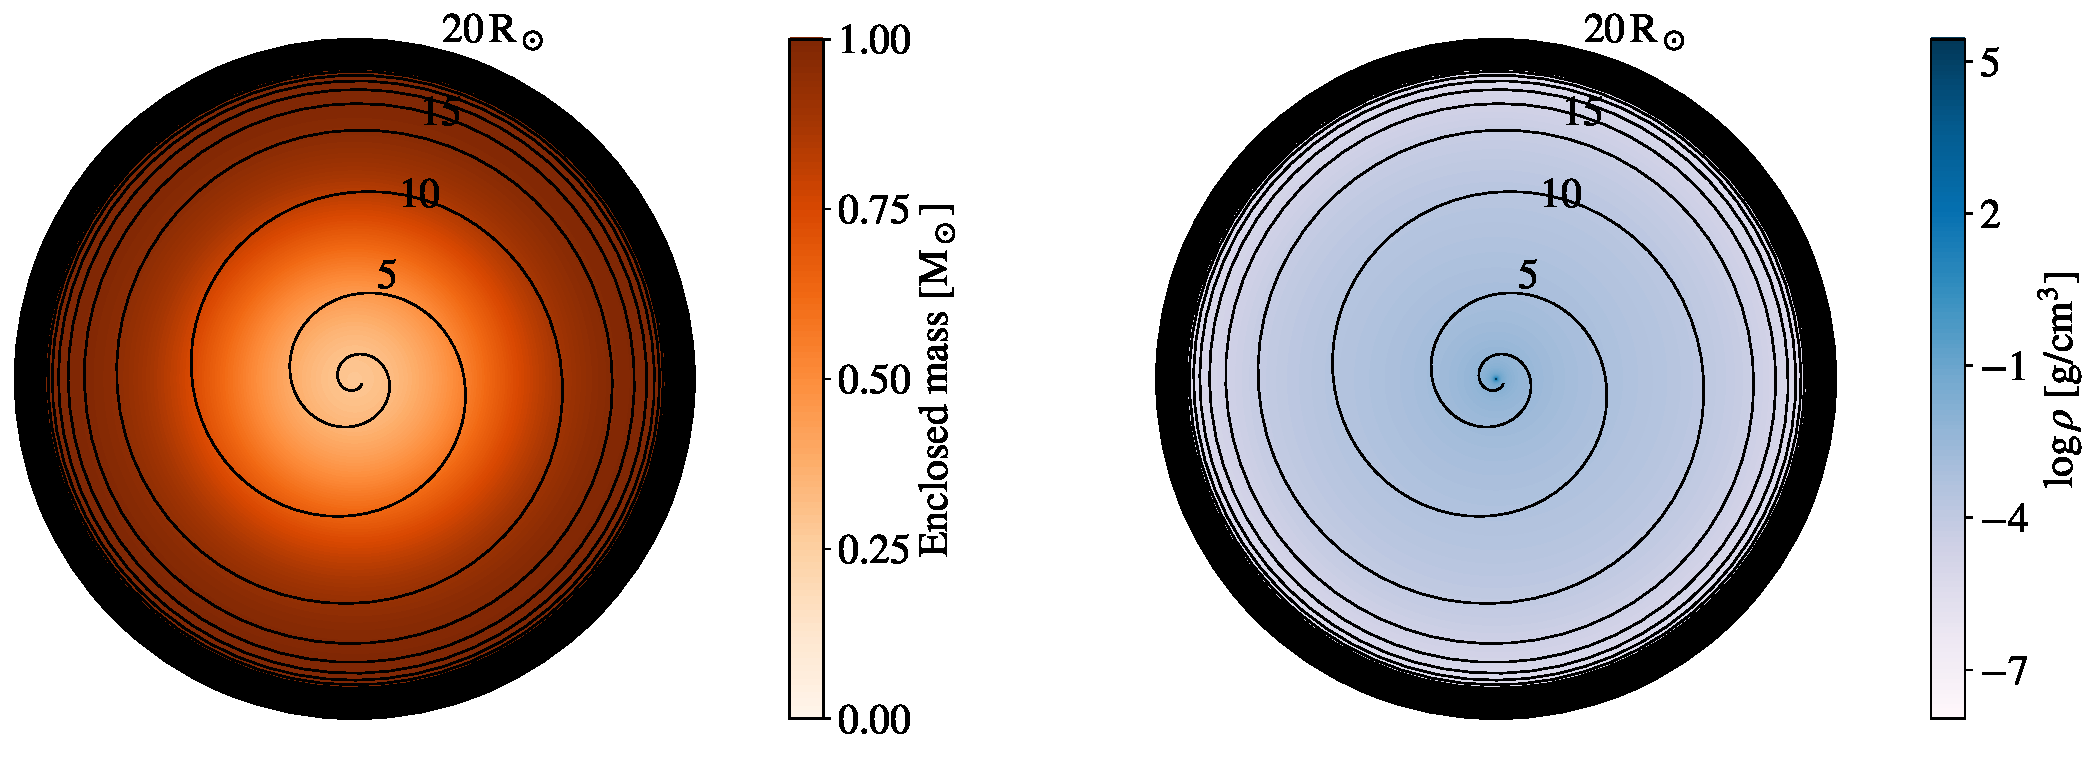
\includegraphics[width=\textwidth]{figures/polar_mj_r20.pdf}
\caption{Engulfment of a planet with Jupiter mass and radius around a red giant star with mass 1$\Msun$ and radius 20$\Rsun$.}
\label{fig:spiral20}
\end{figure*}





\section{Discussion}\label{sec:discussion}
\subsection{Orbital Evolution}\label{sec:orbital_evolution}
 In our models we calculate the orbital evolution in a simplified way, assuming that the planet's relative velocity is always equal to the Keplerian value. This assumption breaks down as the drag force becomes comparable to gravity and the planet starts falling radially. This choice leads to an overestimate of the drag luminosity injected in our model respect to what is happening in a real engulfment event. This said our predictions for the lightcurve associated with the engulfment should not depend too much on this assumption. In particular the early phase of the transient and its maximum brightness are not affected, since  the luminosity  during the grazing and plunge-in phase is coming from the heating of the outer stellar layers. Heating of deeper layers mostly contribute to the stellar luminosity during the long, thermal relaxation phase. 
 
\subsection{Different Destruction Mechanisms}
We adopted the criteria of \citet{Jia_2018}, but other effects could determine the maximum penetration of the planet. While this would change some of the properties of our engulfment calculations, for the same reasons as in \ref{sec:orbital_evolution} we argue that the lightcurve associated with the engulfment events should not be profoundly affected. 
We tested a few models artificially changing the depth of planetary destruction, and found that results do not change substantially (maybe add a figure in Appendix).
\subsection{Rotation}
While the stellar envelope of evolved stars are slowly rotating, an engulfment process is expected to deposit angular momentum and change the rotational properties of the star \citep[see e.g.][]{Privitera:2016a,Privitera:2016b}. Here we have neglected this effect, so we can not track the rotational evolution of the engulfment product. This is the most important short-coming of our models, as the relative velocity of the planet respect to the stellar envelope determines the heating rate and orbital decay (Eq.~\ref{eq:de} and \ref{eq:dr}). We will explore the effects of including the deposition of angular momentum from engulfed planets in future work. 

Together with chemical enrichment \citep[e.g. Lithium, see][]{Soares:2021} rapid rotation and enhanced activity could be observational signatures of an engulfment. The activity is believed to be caused by rapid rotation and convection, which could lead to a dynamo in the stellar envelope \citep{Soker:2007,Privitera:2016bf}

%\subsection{Magnetic Fields}

\subsection{Emission Mechanism and Mass Loss}\label{sec:emission}
Although the early-time peaks
seen in many light curves of Luminous Red Novae (LRN) can be powered by the initial thermal energy of hot ejecta (MacLeod et al.
2017; Metzger \& Pejcha 2017), the longer-lived plateau
emission (sometimes manifesting as a second luminosity
peak) is powered by hydrogen recombination energy or
other forms of radially-distributed ejecta heating (e.g.,
shock interaction between the fast merger ejecta and circumbinary material from the pre-dynamical phase; Metzger \& Pejcha 2017, or from an accretion-powered jet;
e.g., Soker 2020; Soker \& Kaplan 2021).

\subsection{Mass Loss}
In our models we assume that the orbital energy of the planet (kinetic plus gravitational) is injected in the stellar envelope as internal energy via hydrodynamic or gravitational drag. The light curve is then powered by thermal energy of the hot gas.
Of course some of the orbital energy could actually directly go into kinetic energy of stellar material, possibly causing an outflow. Such mechanical perturbation is especially likely to occur in the grazing phase of an engulfment, with the planet potentially able to peel away gas from the outer, least gravitationally bound layers of a star. 
In the presence of an outflow,  the light-curve evolution could also be shaped by energy released from hydrogen recombination \citep{Ivanova:2013}.
Recently \citet{Matsumoto:2022} extended the work of \citet{Ivanova:2013} and explored the parameter space of hydrogen recombination powered merger events, pointing out that for planet-star mergers hydrogen recombination should lead to modest luminosity increase.
Since the amount of mass lost during the merger determines the contribution of hydrogen recombination to the light-curve, we investigated the maximum amount of stellar material that could be unbound using the orbital energy of a planet. For a 1$\Mj$ planet around an evolved 1$\Msun$ star this is about $\sim 5\times10^{-4}\Msun$, increasing to $\sim 5\times10^{-3}\Msun$ for a 10$\Mj$ object (See Fig.~\ref{fig:binding}). These are upper limits to the mass loss, as in reality only a fraction of the orbital energy is going into unbinding envelope material.
However, even a relatively small amount of outflow can contribute substantially to the light-curve via recombination energy, so to create realistic light-curves of planetary merger events one has to combine both the contribution from envelope heating and from outflow recombination. The latter requires a detailed understanding of the mass loss, something that our one-dimensional models can not capture yet. 
% But we could use sims from 
%\citet{Matsumoto:2022} propose that the 



%Looking at the amount of material that was unbound in the watershed merger event V1309Sco \citep{Tylenda:2011}, we can determine what's the likely fraction of the orbital energy contributing to the outflow. In the case of V1309Sco it is believed that about $10^{-2}-10^{-3} \Msun$ of gas was espelled during the event \citep{Tylenda:2016,Matsumoto:2022}. The luminosity and effective temperature of the primary were consistent with a $\approx 1\Msun$ star at the beginning of the red giant branch, and the expected orbital energy of the V1309Sco progenitor system is $0.2-5.6 \times 10^{47}$ erg \citep{Tylenda:2011}. A comparison of this energy with the binding energy of a $\approx 1\Msun$ star at the beginning of the red giant branch shows that the efficiency of the process is on the order 



\begin{figure*}
\centering
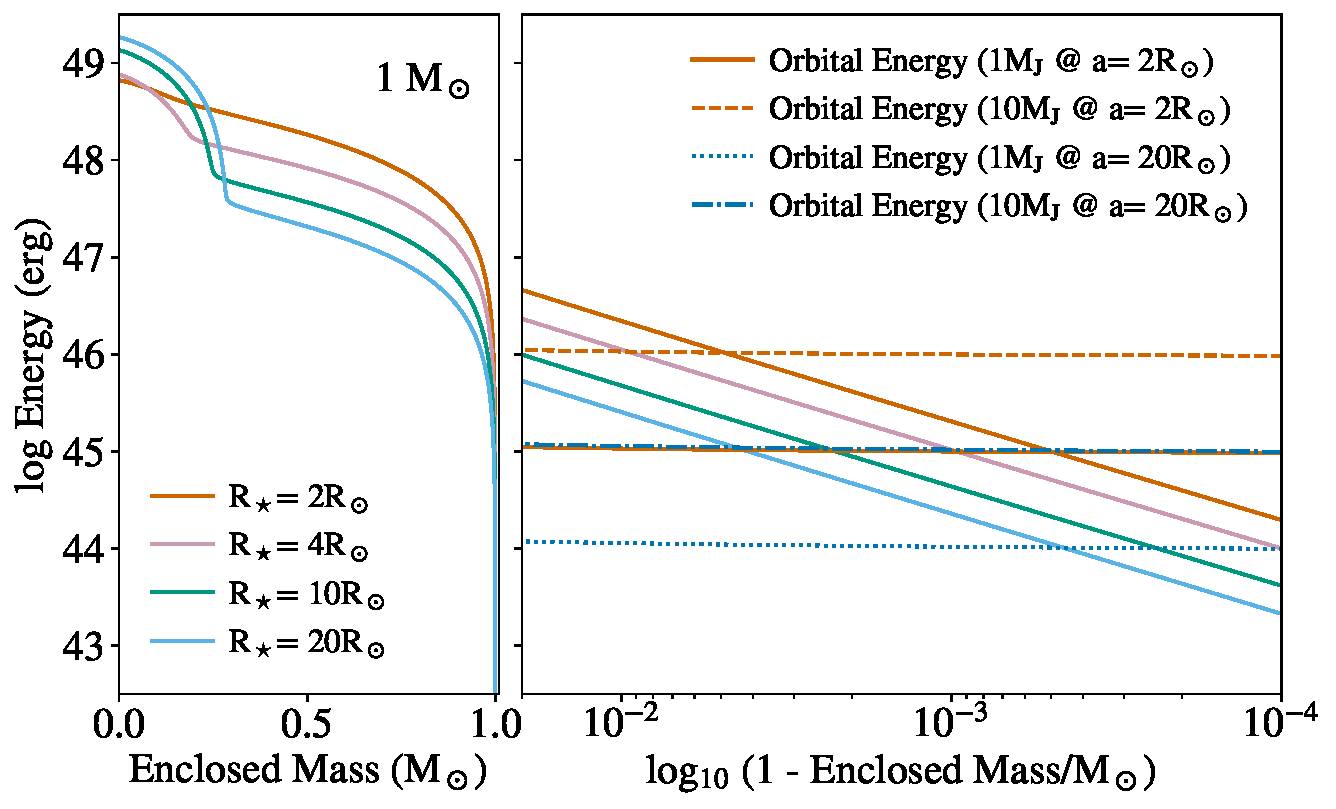
\includegraphics[width=\textwidth]{figures/binding.pdf}
\caption{Binding energy (gravitational minus thermal energy) in the envelope of evolved 1$\Msun$ with different stellar radii. This gravitational binding energy as function of mass coordinate shows the minimum amount of injected energy required to unbind the overlying layers.
The right panel shows a comparison between the binding energy in the outer $\sim 10^{-2}\Msun$ of stellar envelope with the energy (gravitational plus kinetic) available in a planet of 1 and 10 $\Mj$ orbiting the star.}
\label{fig:binding}
\end{figure*}



\section{Conclusions}

\acknowledgments
The Center for Computational Astrophysics at the Flatiron Institute is supported by the Simons Foundation.

\bibliographystyle{aasjournal}
\bibliography{biblio.bib}

\end{document}


